\chapter{Results}

The central focus of this project was to develop a pipeline to identify structured RNA elements and to apply this in the search of candidate light-responsive RNA elements (or ``light switches'').


\section{Positive control search: Can protein homology be rediscovered from known \ac{RNP}s?}

% go through fmn riboswitch, other riboswitches and crispr examples briefly
The hypothesis on which this work is based is that protein homology can be leveraged to identify RNA homology in \ac{RNP} systems, on the basis that they are encoded at neighbouring loci.
Approaching the hypothesis from the other direction, the positive control pipeline described in Figure~\ref{fig:poscontrol} searches for protein homology in coding sequences neighbouring known RNA family members.
Clustering of neighbouring protein sequences was used as a proxy for homology.

\begin{table}[H]
\centering
\footnotesize
\caption[Top cluster for each RNA family]{\textbf{Top cluster (by genome prevalence) for each RNA family} }
    \label{tab:results_summary}
    
\begin{tabular}{p{0.18\textwidth}p{0.08\textwidth}p{0.17\textwidth}p{0.30\textwidth}p{0.16\textwidth}}
\hline
\textbf{RNA family} & \textbf{Cluster} & \textbf{Genomes (prevalence)} & \textbf{Top Pfam InterProScan hit (\% of cluster sequences)$^{*}$} & \textbf{Dominant position (\% sequences)$^{**}$} \\
\hline
FMN riboswitch (RF00050) & 204 & 926/2009 (46.1\%) & RibD C-terminal domain (100\%) & Upstream 1 (97.9\%) \\
SAM riboswitch (RF00162) & 831 & 634/1535 (41.3\%) & Cys/Met metabolism PLP-dependent enzyme (100\%) & Upstream 1 (97.6\%) \\
CRISPR-DR42 (RF01351) & 294 & 28/65 (43.1\%) & CRISPR-associated protein Cas2 (100\%) & Downstream 1 (98.9\%) \\
Fluoride riboswitch (RF01734) & 761 & 259/661 (39.2\%) & CrcB-like protein, camphor resistance (100\%) & Upstream 1 (93.9\%) \\
\hline
\end{tabular}
    \par\smallskip
    \begin{minipage}{\textwidth}
        \raggedright
        $^{*}$ Prevalence is the fraction of available genomes containing the cluster.\\
        $^{**}$ Position is given as strand-relative direction and gene rank (e.g.\ upstream 1 = RNA element immediately upstream of the cluster gene).
    \end{minipage}
\end{table}

Using protein clustering by alignment to infer protein homology in neighbouring coding sequences of RNA family members, the positive control pipeline was able to rediscover known \ac{RNP} systems (Table~\ref{tab:results_summary}).
The \ac{FMN} riboswitch, \ac{SAM} riboswitch, \ac{CRISPR}-DR42 and Fluoride riboswitch were all found to be associated with particular conserved protein domains, RibD C-terminal domain, Cys/Met metabolism PLP-dependent enzyme, CRISPR-associated protein Cas2 and CrcB-like protein camphor resistance, respectively.
These protein domains were identified in the highest prevalence cluster of coding sequences neighbouring the RNA family members, and the position of the RNA element relative to the protein-coding gene was consistent with known biology \citep{Mironov2002}.

\section{Can RNA homology be rediscovered from known \ac{RNP}s?}

A selection of riboswitches and the \ac{CRISPR} repeat element were found to be associated with particular conserved protein domains.
With this direction shown it remains to show that RNA homology can be identified anchoring the search with a conserved protein.
Any of these could presumably be used for validation of the computational discovery pipeline.
The \ac{CRISPR}-Cas system would be interesting to validate; however, in its current state the discovery pipeline extracts only intergenic regions on the same strand as the protein anchor.
Further, the prevalence of the \ac{RNP} and genome availability (limited by Rfam and Entrez entries) were deciding factors.
As such, the \ac{FMN} riboswitch and its associated protein domain, the RibD C-terminal domain, were used for positive control validation.

\subsection{\ac{FMN} riboswitch as a positive control}
% explain rna -> protein -> rna idea for val

The RibD C-terminal domain, with a profile \ac{HMM} generated in the positive control preparation pipeline (Section~\ref{sec:positive_control_hmm}), was used as an anchor to investigate if the \ac{FMN} riboswitch signal could be rediscovered.
The bacterial family Microbacteriaceae was used as a search space, informed by the phylogenetic distribution of the riboswitch and protein pairing found in the positive control preparation pipeline (Appendix Figure \ref{fig:fmn-itol-tree}).
726 loci were identified in the \emph{Microbacteriaceae} search space (697 genomes), when searched with the curated \ac{FMN} Riboswitch model, E-value $< 1\times10^{-5}$. 
Of these 726 loci, 613 were found in the identified anchor-domain flanking regions.
10 out of 13 candidates of the discovery pipline were able to identify (with at least some overlap) all 613 loci.
The outputs of the discovery pipeline were run through the iterative expansion approach described in Section~\ref{sec:iterative}, and the resulting alignments were analysed for covariation with R-scape \citep{Rivas2017} and compared to the true-positive alignment identified with the Rfam curated \ac{FMN} Riboswitch model.
Pipeline thresholds for this run are defined in Appendix Table~\ref{tab:thresholds}.
The resulting candidates are shown in Table~\ref{tab:rscape_summary}, ordered by coordinate overlap identity with the true-positive alignment, along with their covariation analysis F-scores and median summed bit scores against the curated \ac{FMN} Riboswitch model.

\begin{table}[H]
\centering
\footnotesize
\caption[FMN riboswitch rediscovery candidates]{\textbf{FMN riboswitch rediscovery candidates.}
    A summary of the candidate strucutred elements identified by the discovery and iterative expansion pipelines, and their covariation analysis results.
    Candidates are compared to a true-positive alignment and model to assess their recovery of the known \ac{FMN} riboswitch signal.}
\label{tab:rscape_summary}
\begin{tabular}{cccc}
\hline
\textbf{Candidate} & \textbf{F-score$^{*}$} & \textbf{\% overlap identity$^{\dagger}$} & \textbf{Summed median score (bits)$^{\ddagger}$} \\
\hline
416 & 78.95 & 76.75 & 36.35 \\
647 & 73.17 & 67.99 & 47.45 \\
35  & 62.07 & 75.02 & 52.55 \\
379 & 61.18 & 80.36 & 61.30 \\
491 & 60.67 & 67.95 & 45.20 \\
40  & 56.67 & 74.41 & 38.15 \\
384 & 55.70 & 68.73 & 38.95 \\
539 & 53.85 & 76.99 & 32.45 \\
531 & 48.15 & 78.73 & 34.35 \\
396 & 34.04 & 0.00  & 3.20 \\
109 & 32.26 & 0.00  & 3.00 \\
442 & 20.00 & 0.00  & $-0.60$ \\
\hline
\end{tabular}

\vspace{4pt}
\begin{minipage}{\textwidth}
\raggedright
$^{*}$ R-scape F-score for recovery of covarying base pairs relative to the secondary structure annotated within each candidate's own alignment, at $E \le 0.05$.\\
$^{\dagger}$ Mean coordinate overlap (intersection/union) of the hits shared between the candidate and the true-positive alignment.\\
$^{\ddagger}$ Sum of the median \texttt{cmsearch} bit scores of synthesised candidate sequences scored against the \ac{FMN} Riboswitch model and synthesised \ac{FMN} Riboswitch sequences scored against the candidate model ($N = 300$ emitted sequences per model).
\end{minipage}
\end{table}

Table \ref{tab:rscape_summary} shows 9 candidates with a mean coordinate overlap of $>0.67$ with the true-positive alignment, and summed median bit scores of $>32$.
This suggests that the candidates identify largely the same genomic loci as the true-positive alignment, and that their probabilistic models describe much of the same structural information.
Secondary structures were predicted for all candidates and the top two, by highest coordinate overlap identity to the true-positive alignment, are shown in Figure~\ref{fig:drh-top-structures}.
The predicted structures of the remaining candidates are shown in Appendix Figure~\ref{fig:drh-appendix-structures-1}.

\begin{figure}[H]
    \centering

    % ---- Row 1: (a) and (b) ----
    \begin{subfigure}[t]{0.48\textwidth}
        \centering
        \caption{Rfam consensus structure}
        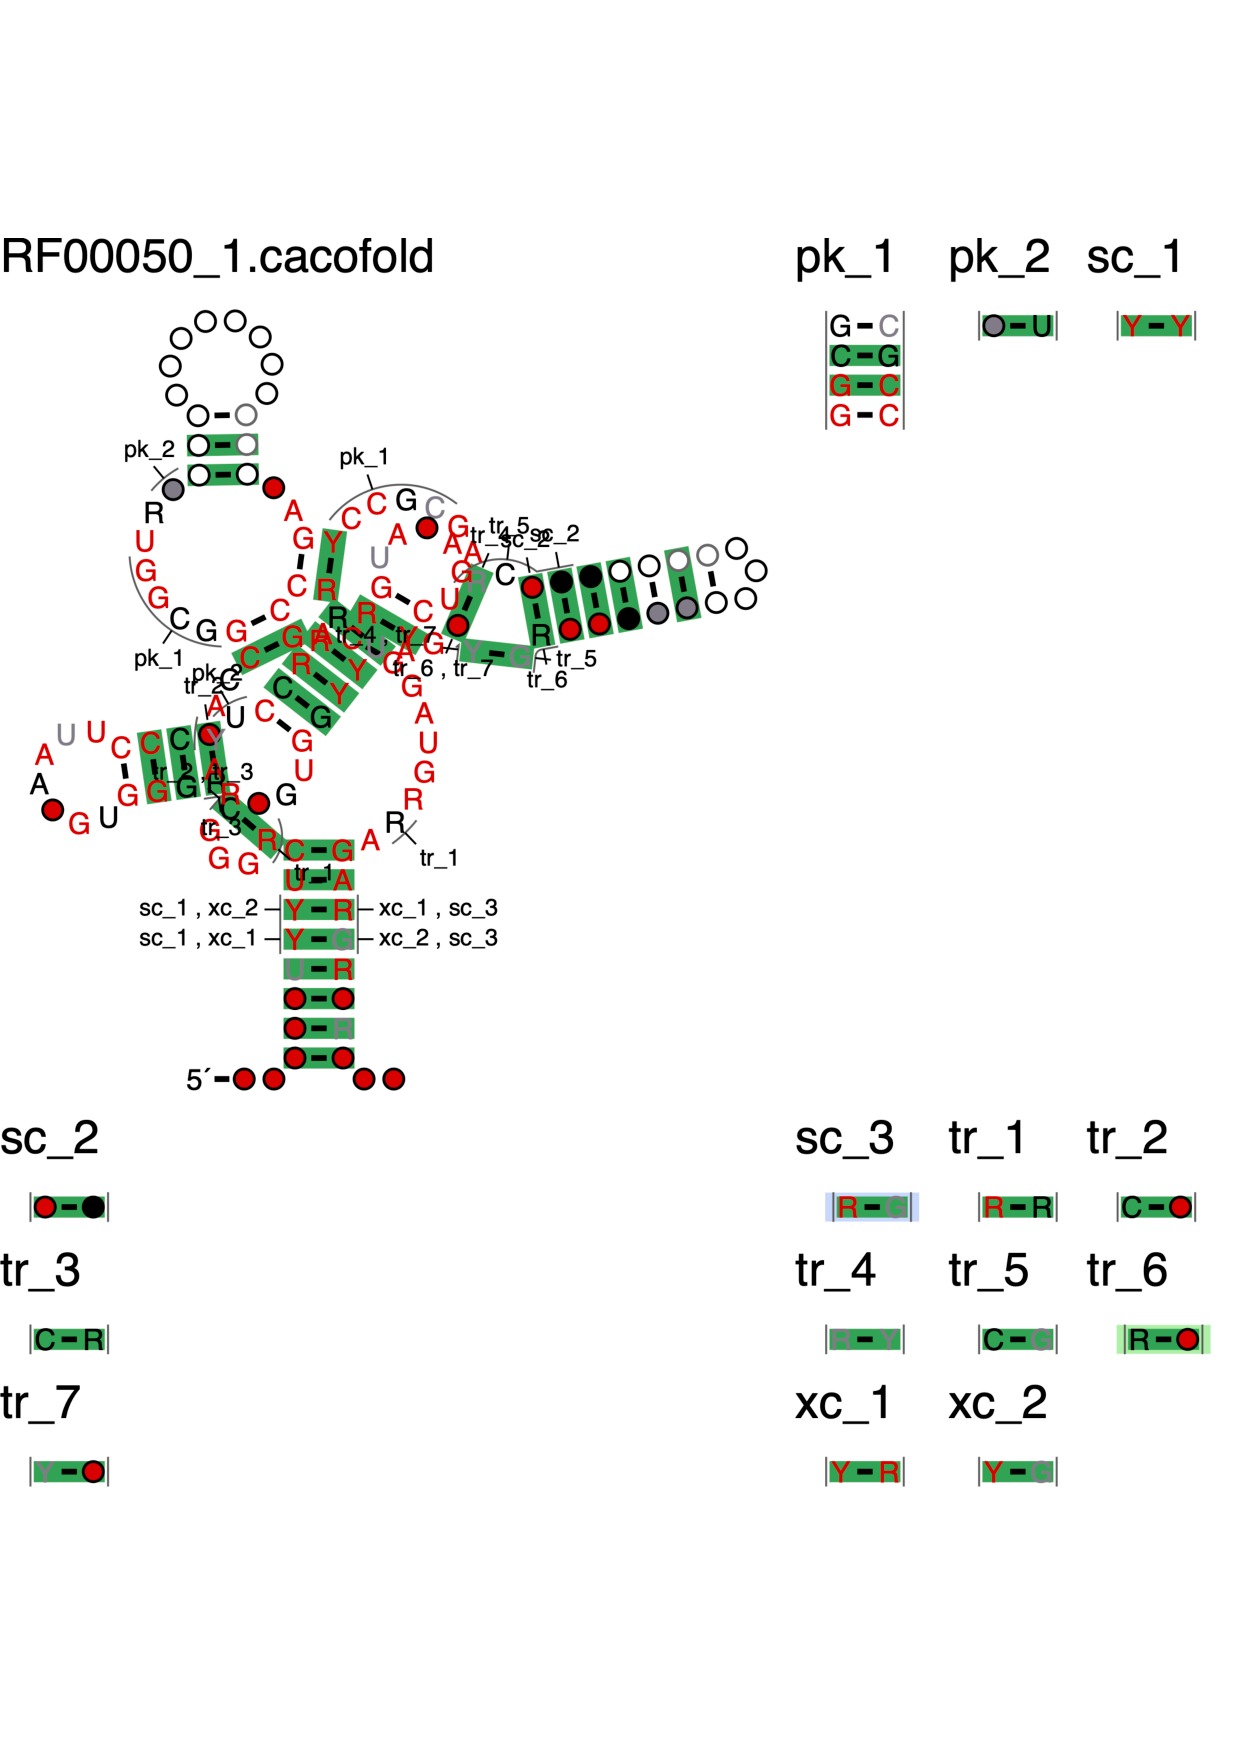
\includegraphics[width=\linewidth, height=0.3\textheight, keepaspectratio]{figures/results/RF00050_1.cacofold.R2R.sto.pdf}
        \label{fig:rfam-consensus-struct}
    \end{subfigure}
    \hfill
    \begin{subfigure}[t]{0.48\textwidth}
        \centering
        \caption{Positive control}
        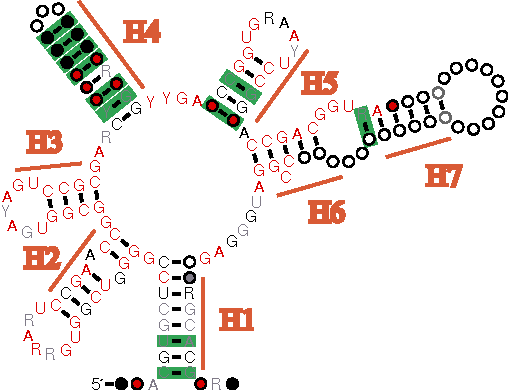
\includegraphics[width=\linewidth, height=0.3\textheight, keepaspectratio]{figures/results/drh-iteritive-expansion-structures/fmn_cm_on_micro_1.cacofold.R2R.sto.pdf}
        \label{fig:cand-positive-control-struct}
    \end{subfigure}

    \vspace{1em}

    % ---- Row 2: two candidates ----
    \begin{subfigure}[t]{0.48\textwidth}
        \centering
        \caption{Candidate 379}
        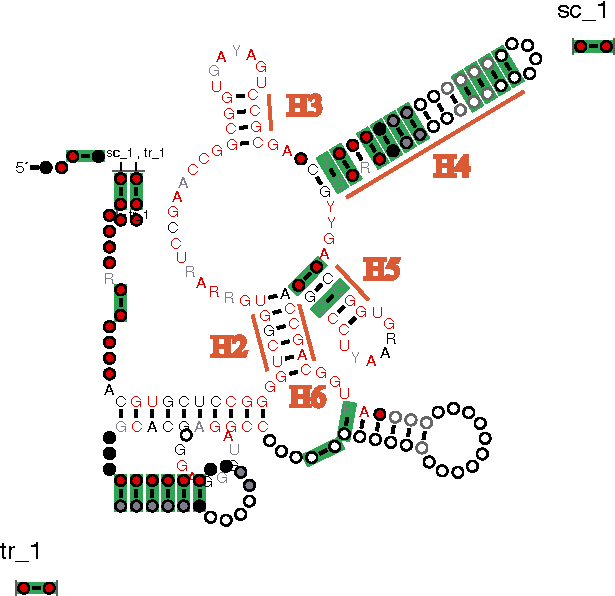
\includegraphics[width=\linewidth, height=0.3\textheight, keepaspectratio]{figures/results/drh-iteritive-expansion-structures/cluster_379_alignment_02_1.cacofold.R2R.sto.pdf}
        \label{fig:cand379-struct}
    \end{subfigure}
    \hfill
    \begin{subfigure}[t]{0.48\textwidth}
        \centering
        \caption{Candidate 531}
        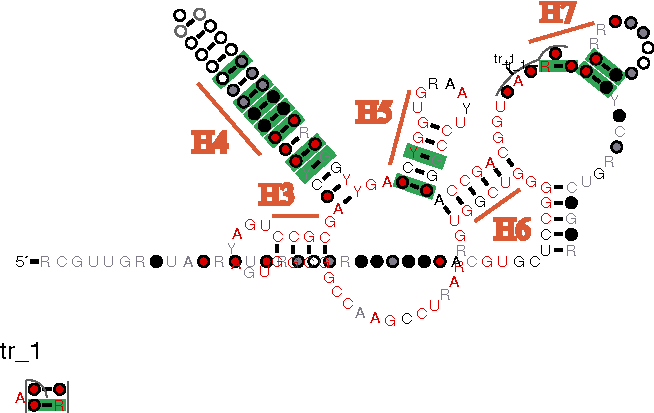
\includegraphics[width=\linewidth, height=0.3\textheight, keepaspectratio]{figures/results/drh-iteritive-expansion-structures/cluster_531_alignment_02_1.cacofold.R2R.sto.pdf}
        \label{fig:cand531-struct}
    \end{subfigure}


    \caption[Predicted covarying secondary structures of positive control candidates]{\textbf{Predicted covarying secondary structures of top two FMN riboswitch candidates by highest coordinate overlap identity to the positive control.}
    R-scape CaCoFold structures generated from iteratively expanded alignments, ranked by mean coordinate overlap (intersection/union) of hits shared with the true-positive alignment.
    Annotated H1-H7 are the seven helices similar across the different structures.
    \textbf{(a)}: the Rfam \ac{FMN} riboswitch consensus structure, for reference;
    \textbf{(b)}: the true-positive alignment (\texttt{fmn\_cm\_on\_micro}), made from the same flanking sequences as the candidates and identified by searching with the Rfam \ac{FMN} riboswitch model i.e. the best signal that could have been recovered.;
    \textbf{(c)} and \textbf{(d)}: the two candidates with highest overlap identity to the true-positive alignment.}
    \label{fig:drh-top-structures}
\end{figure}

The CaCoFold predicted structures of the two candidates with highest coordinate overlap identity to the true-positive alignment (Figure~\ref{fig:drh-top-structures}) illustrate the presence of covarying base pairs in the same regions as the true-positive alignment, and the overall secondary structure is similar.
Shown for reference in this figure is the consensus structure of the \ac{FMN} riboswitch, as annotated in Rfam, and the positive control alignment, which was made from the same flanking sequences as the candidates and identified by searching with the Rfam \ac{FMN} riboswitch model.
As can be seen from the annotated helices, the predicted structures of the candidates are similar to the positive alignment and the Rfam consensus structure, with some variation in the number of helices and their lengths.
Candidates 379 and 531 (figures \ref{fig:cand379-struct} and \ref{fig:cand531-struct}) have predicted structures with many of the same helices as the positive control and Rfam consensus structure.
Interestingly, candidate 379 (Figure~\ref{fig:cand379-struct}) has a predicted structure with a hybrid H2-H6 helix, which is not present in the positive control or Rfam consensus structure.
This could represent an alternative conformation of the riboswitch, but it may also be an artefact of the alignment and would require further testing.

It should be noted that this is a single, relatively easy positive control.
The \ac{FMN} riboswitch is highly conserved and well characterised, and the protein domain profile used as the anchor was generated from sequences neighbouring the Rfam-annotated riboswitch.
Recovery of this signal is therefore a best-case scenario for the pipeline, rather than a general measure of its sensitivity.

\subsection{Negative control}
% explain choice of 

Four membrane-associated protein domains were chosen as negative controls on the basis that they were unlikely to be involved in \ac{RNP} systems (Section~\ref{sec:negative-control}).
These were the SecY protein translocase, the YgaP-like inner membrane protein, the YadA-like, C-terminal domain outer membrane protein and the Bacterial flagellin N-terminal domain.
Surprisingly, the flagellin domain returned promising structured RNA candidates from the computational discovery pipeline and was excluded from the negative control set; the resulting candidates are shown in Appendix Table~\ref{tab:flagellin_appendix}. 
Nine candidates were identified with F-scores ranging from 1.2 to 43.14, indicating a moderate level of structural signal.
 [NOTE: excluding the one domain that gave a positive result after the fact needs justification here. Say how many candidates it gave and their F-scores, and discuss whether it reflects a real element rather than a failed control.]
The search space for all was the genus \emph{Burkholderia}, which was chosen as all four domains are present in this genus.

\begin{table}[H]
\centering
\footnotesize
\caption[Negative control candidates]{\textbf{Negative control candidates.}
    The SecY protein translocase (IPR002208, PF00538) and the YgaP-like inner membrane protein (IPR021309, PF03471) were screened in both directions and produced clusters with significant covarying pairs ($E \le 0.05$).
    YadA-like membrane anchor domain (IPR005594, PF03895) was also screened in both directions but produced no clusters with a significant covarying pair.
}
\label{tab:negative_control_candidates}
    \begin{tabular}{p{0.10\textwidth}p{0.12\textwidth}p{0.10\textwidth}p{0.12\textwidth}p{0.10\textwidth}p{0.10\textwidth}}
\hline
\textbf{Label} & \textbf{IPR} & \textbf{Candidate} & \textbf{Direction} & \textbf{Cov.\ pairs$^{*}$} & \textbf{F-score} \\
\hline
SecY & IPR002208 & 26 & Downstream & 1 & 6.06 \\
SecY & IPR002208 & 98 & Downstream & 1 & 4.44 \\
YgaP-like & IPR021309 & 90 & Downstream & 2 & 5.63 \\
Flagellin & IPR001029 & 327$^{\dagger}$ & Downstream & 11 & 43.14 \\
Flagellin & IPR001029 & 545 & Downstream & 2 & 8.00 \\
Flagellin & IPR001029 & 589 & Downstream & 4 & 7.48 \\
Flagellin & IPR001029 & 265 & Downstream & 1 & 5.41 \\
Flagellin & IPR001029 & 16 & Upstream & 1 & 4.76 \\
Flagellin & IPR001029 & 725 & Downstream & 1 & 4.35 \\
Flagellin & IPR001029 & 161 & Downstream & 1 & 2.56 \\
Flagellin & IPR001029 & 272 & Downstream & 1 & 2.50 \\
Flagellin & IPR001029 & 214 & Upstream & 1 & 1.20 \\
\hline
\end{tabular}


\par\smallskip
\begin{minipage}{\textwidth}
\raggedright
$^{*}$ Number of covarying base pairs identified by R-scape at $E \le 0.05$; equal to true positives (TP) since FP\,=\,0 in all cases.\\
\end{minipage}
\end{table}

Of the three negative control domains, only the SecY and YgaP-like inner membrane protein domains returned candidates with at least one covarying pair, E-value $\leq 0.05$.
Of these the F-scores are low, and the number of covarying pairs is small, compared to the positive control candidates, suggesting that these are weak signals, consistent with a selective pipeline, although only a small number of negative control domains were tested. [NOTE: give the actual F-scores and pair counts for the negative controls in the text, since the BLUF candidates are compared against them later.]
These results outline expected behaviour of the discovery pipeline when applied to protein domains that are unlikely to be associated with structured RNA elements, and provide a baseline for comparison with the positive control results.

\section{\ac{BLUF} domain \ac{RNP} search}

Having tested the discovery pipeline with positive and negative controls, the pipeline was applied to the \ac{BLUF} domain, which is a light-responsive protein domain.
The \ac{BLUF} domain anchored search was conducted in \emph{Burkholderia}, as this genus contains 701 \ac{BLUF} domain-containing protein sequences \citep{Blum2025}.

\subsection{Identified candidates}

% show the promising structures, table of covarying pairs, alphafold predictions
The discovery pipeline identified two promising structured RNA candidates, Candidate 130 and Candidate 332, which were found in the downstream flanking sequences of \ac{BLUF} domain-containing proteins. [NOTE: state how many candidates the pipeline produced in total and the criteria used to call these two promising, ideally set before looking at the results, otherwise selection bias is a concern.]
These candidates were additionally analysed with the iterative expansion approach described in Section~\ref{sec:iterative}, and the resulting alignments were analysed for covariation with R-scape \citep{Rivas2020}.

\begin{table}[H]
\centering
\footnotesize
\caption[Covariation analysis for the two BLUF-associated candidates]{\textbf{Covariation analysis for the two BLUF-associated candidates, before and after iterative expansion of the covariance model.}}
\label{tab:bluf_rscape}
    \begin{tabular}{p{0.10\textwidth}p{0.14\textwidth}p{0.12\textwidth}p{0.08\textwidth}p{0.10\textwidth}p{0.10\textwidth}}
\hline
\textbf{Candidate} & \textbf{Stage} & \textbf{Cov.\ pairs$^{*}$} & \textbf{F-score} \\
\hline
130 & Pre-expansion  & 4 & 11.27 \\
130 & Post-expansion & 0 & 0.00 \\
332 & Pre-expansion  & 1 & 2.33 \\
332 & Post-expansion & 2 & 5.00 \\
\hline
\end{tabular}

\par\smallskip
\begin{minipage}{\textwidth}
\raggedright
$^{*}$ Number of covarying base pairs identified by R-scape at $E \le 0.05$; equal to true positives (TP) since FP\,=\,0 in all cases.
\end{minipage}
\end{table}

Iterative expansion yielded more sequences for both Candidate 130 and 332; the number of covarying base pairs decreased for Candidate 130 from 4 to none, and increased for Candidate 332 from 1 to 2; similarly, the F-score increased for Candidate 332 and decreased for Candidate 130 (Table~\ref{tab:bluf_rscape}).
This indicates that the original alignment for Candidate 130 better describes a structured element, while the iterative expansion approach improved the alignment for Candidate 332.
Therefore, the iterative expansion approach was used for Candidate 332, while the original alignment was used for Candidate 130 in subsequent analyses. [NOTE: choosing whichever alignment scores better for each candidate adds analytic flexibility. State this as a limitation, or report both versions for both candidates.]

R-scape F-measure is a harmonic mean of sensitivity and positive predictive value, and is an imperfect measure of the strength of covariation signal in an alignment.
With F-scores of 11.27 and 5.00, respectively, both candidates show some evidence of covariation, but compared with the negative control candidates, the signal is weak, particularly for Candidate 332.
Another measure of covariance is to look at the number of covarying base pairs.
The 4 and 2 covarying base pairs ($E \le 0.05$) identified for these candidates are higher than the counts for the negative control candidates, suggesting there may be some structural signal present. [NOTE: the two lines of evidence point in opposite directions (weak F-scores versus more covarying pairs than the negative controls). Say plainly which you weight and why. Also note that Candidate 130 has no covarying pairs after expansion, so the 4 pairs refer to its original alignment.]
Predicted secondary structures are shown in Figure~\ref{fig:bluf-rscape-structure}.

Candidate sequences were also searched against the Rfam database \citep{Ontiveros-Palacios2025} to identify any known RNA families.
The annotated family inclusion cutoffs of each model were used to determine if a candidate sequence was a member of a known RNA family. [NOTE: Rfam inclusion (gathering) cutoffs are bit scores rather than E-values. Describe this search (tool, database version, cutoff type) in Methods.]
Neither candidate was found to be a member of any known RNA family.

\begin{figure}[H]
    \centering
    \begin{subfigure}
        [t]{0.45\textwidth}
        \centering
        \caption{Candidate 130} \label{fig:cand130-secondary}
        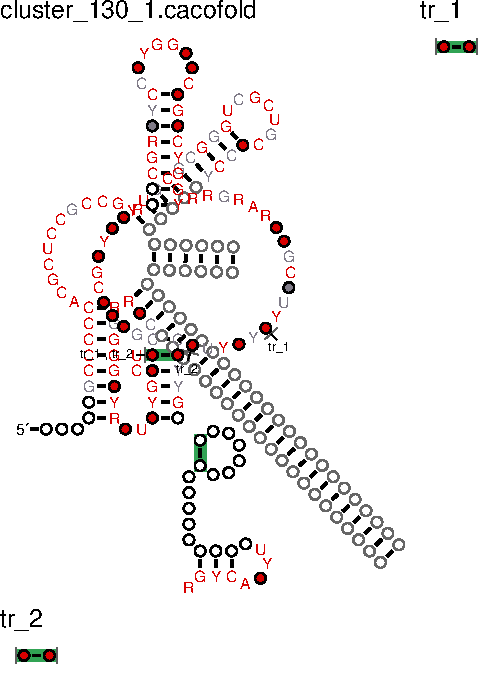
\includegraphics[width=\linewidth, height=0.4\textheight, keepaspectratio]{figures/results/bluf-candidate-structures/cluster_130_1.cacofold.R2R.sto.pdf} 
    \end{subfigure}
    \begin{subfigure}
        [t]{0.45\textwidth}
        \centering
        \caption{Candidate 332} \label{fig:cand332-secondary}
        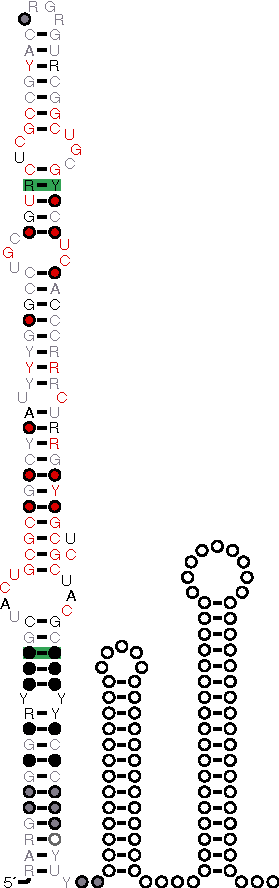
\includegraphics[width=\linewidth, height=0.4\textheight, keepaspectratio]{figures/results/bluf-candidate-structures/cluster_332_alignment_02_1.cacofold.R2R.sto.pdf} 
    \end{subfigure}
    \caption[Predicted covarying secondary structures of the two BLUF-associated candidates]{\textbf{Predicted covarying secondary structures of the two BLUF-associated candidates.}
    Predicted covarying secondary structures of the two most promising structured RNA elements identified through the discovery pipeline.
    Structures are generated by R-scape CaCoFold.
    \textbf{(a)}: shows the predicted secondary structure of candidate 130 as output by the computational discovery pipeline described in the methods,
    \textbf{(b)}: shows that for candidate 332 run through the iterative expansion approach described in the methods.}
    \label{fig:bluf-rscape-structure}
\end{figure}

Candidate 130 shows some promise for an alternative structure with a conserved CGGCG and GCCGC sequence not predicted to base pair in the CaCoFold structure, but which could form a stem-loop structure with covarying base pairs. [NOTE: support this with an alignment excerpt, or by testing the proposed stem-loop for covariation with R-scape.]


\subsection{\ac{RNP} complex prediction}

3D structure and interaction prediction was done with AlphaFold 3 \citep{Abramson2024} (Section~\ref{sec:alphafold}) using the highest-confidence model for each candidate (as determined by the model's predicted confidence score).
Sequences for the following predictions are shown in Appendix Table~\ref{tab:rna_protein_3d_inputs}.

\begin{figure}[H]
    \centering
    \begin{subfigure}
        [t]{0.6\textwidth}
        \centering
        \caption{Candidate 130} \label{fig:cand130-bluf}
        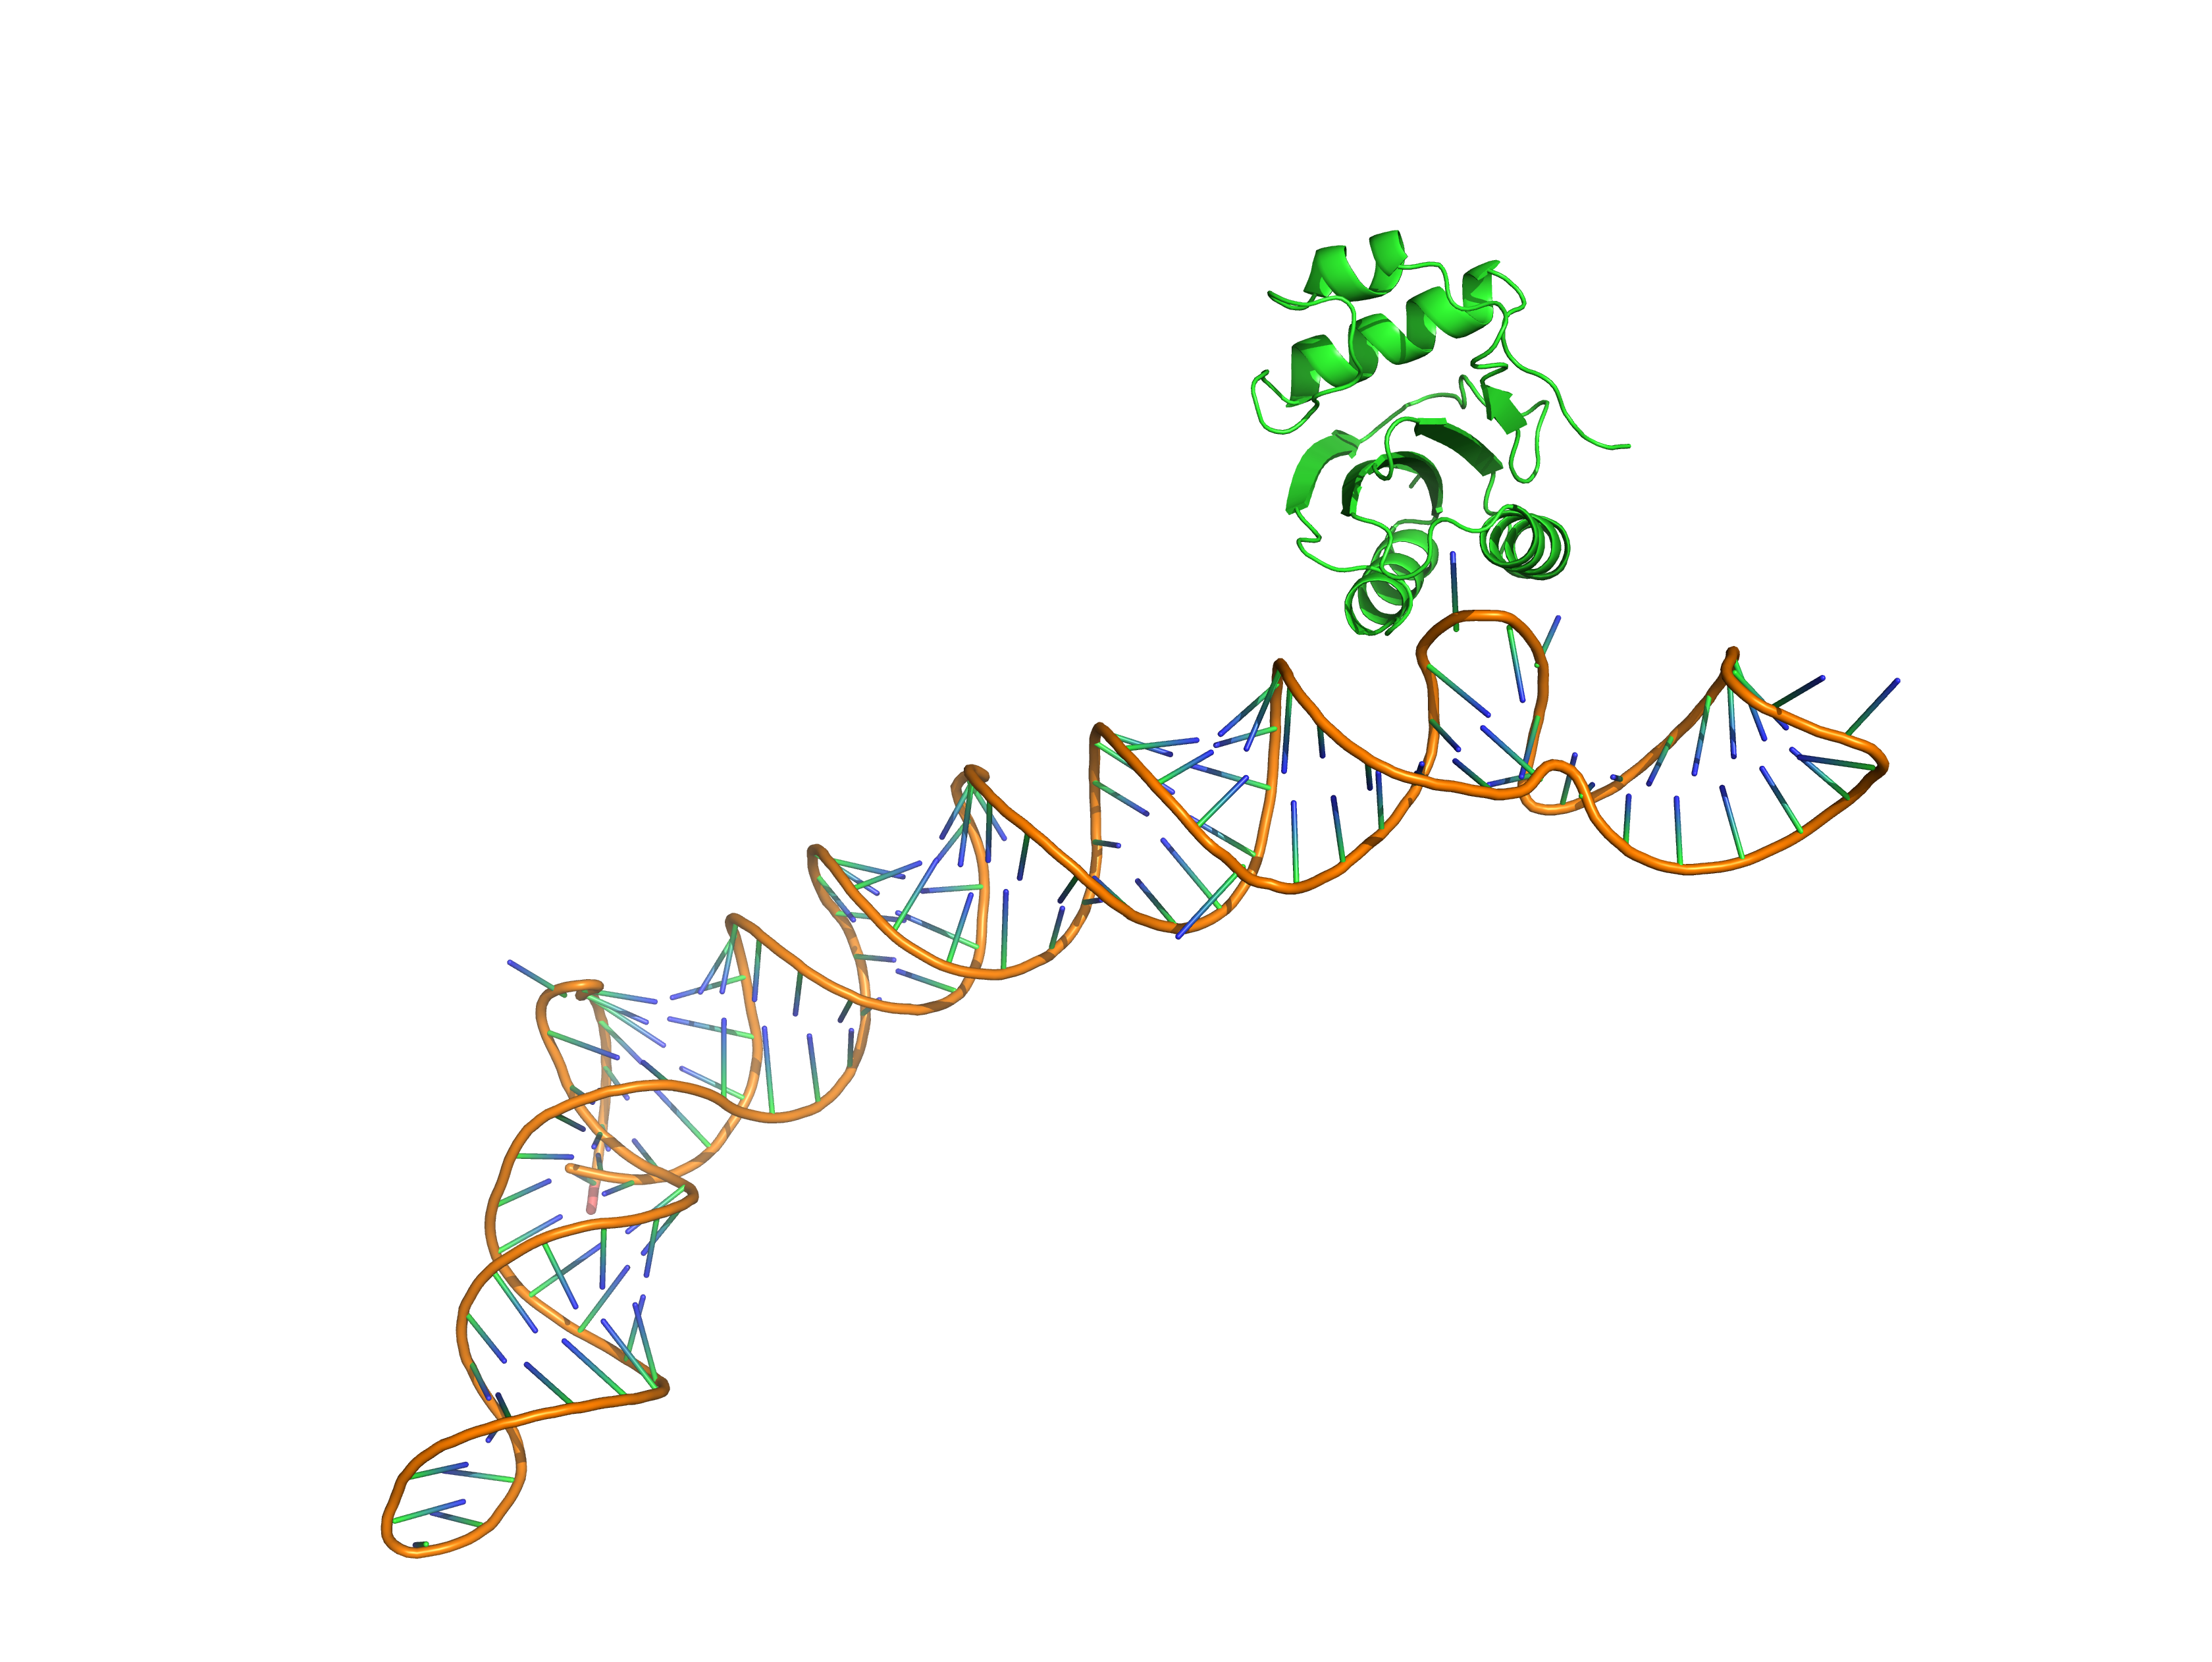
\includegraphics[width=\linewidth]{figures/results/cand130-BLUF-struct.png} 
    \end{subfigure}
    \begin{subfigure}
        [t]{0.6\textwidth}
        \centering
        \caption{Candidate 332} \label{fig:cand332-bluf}
        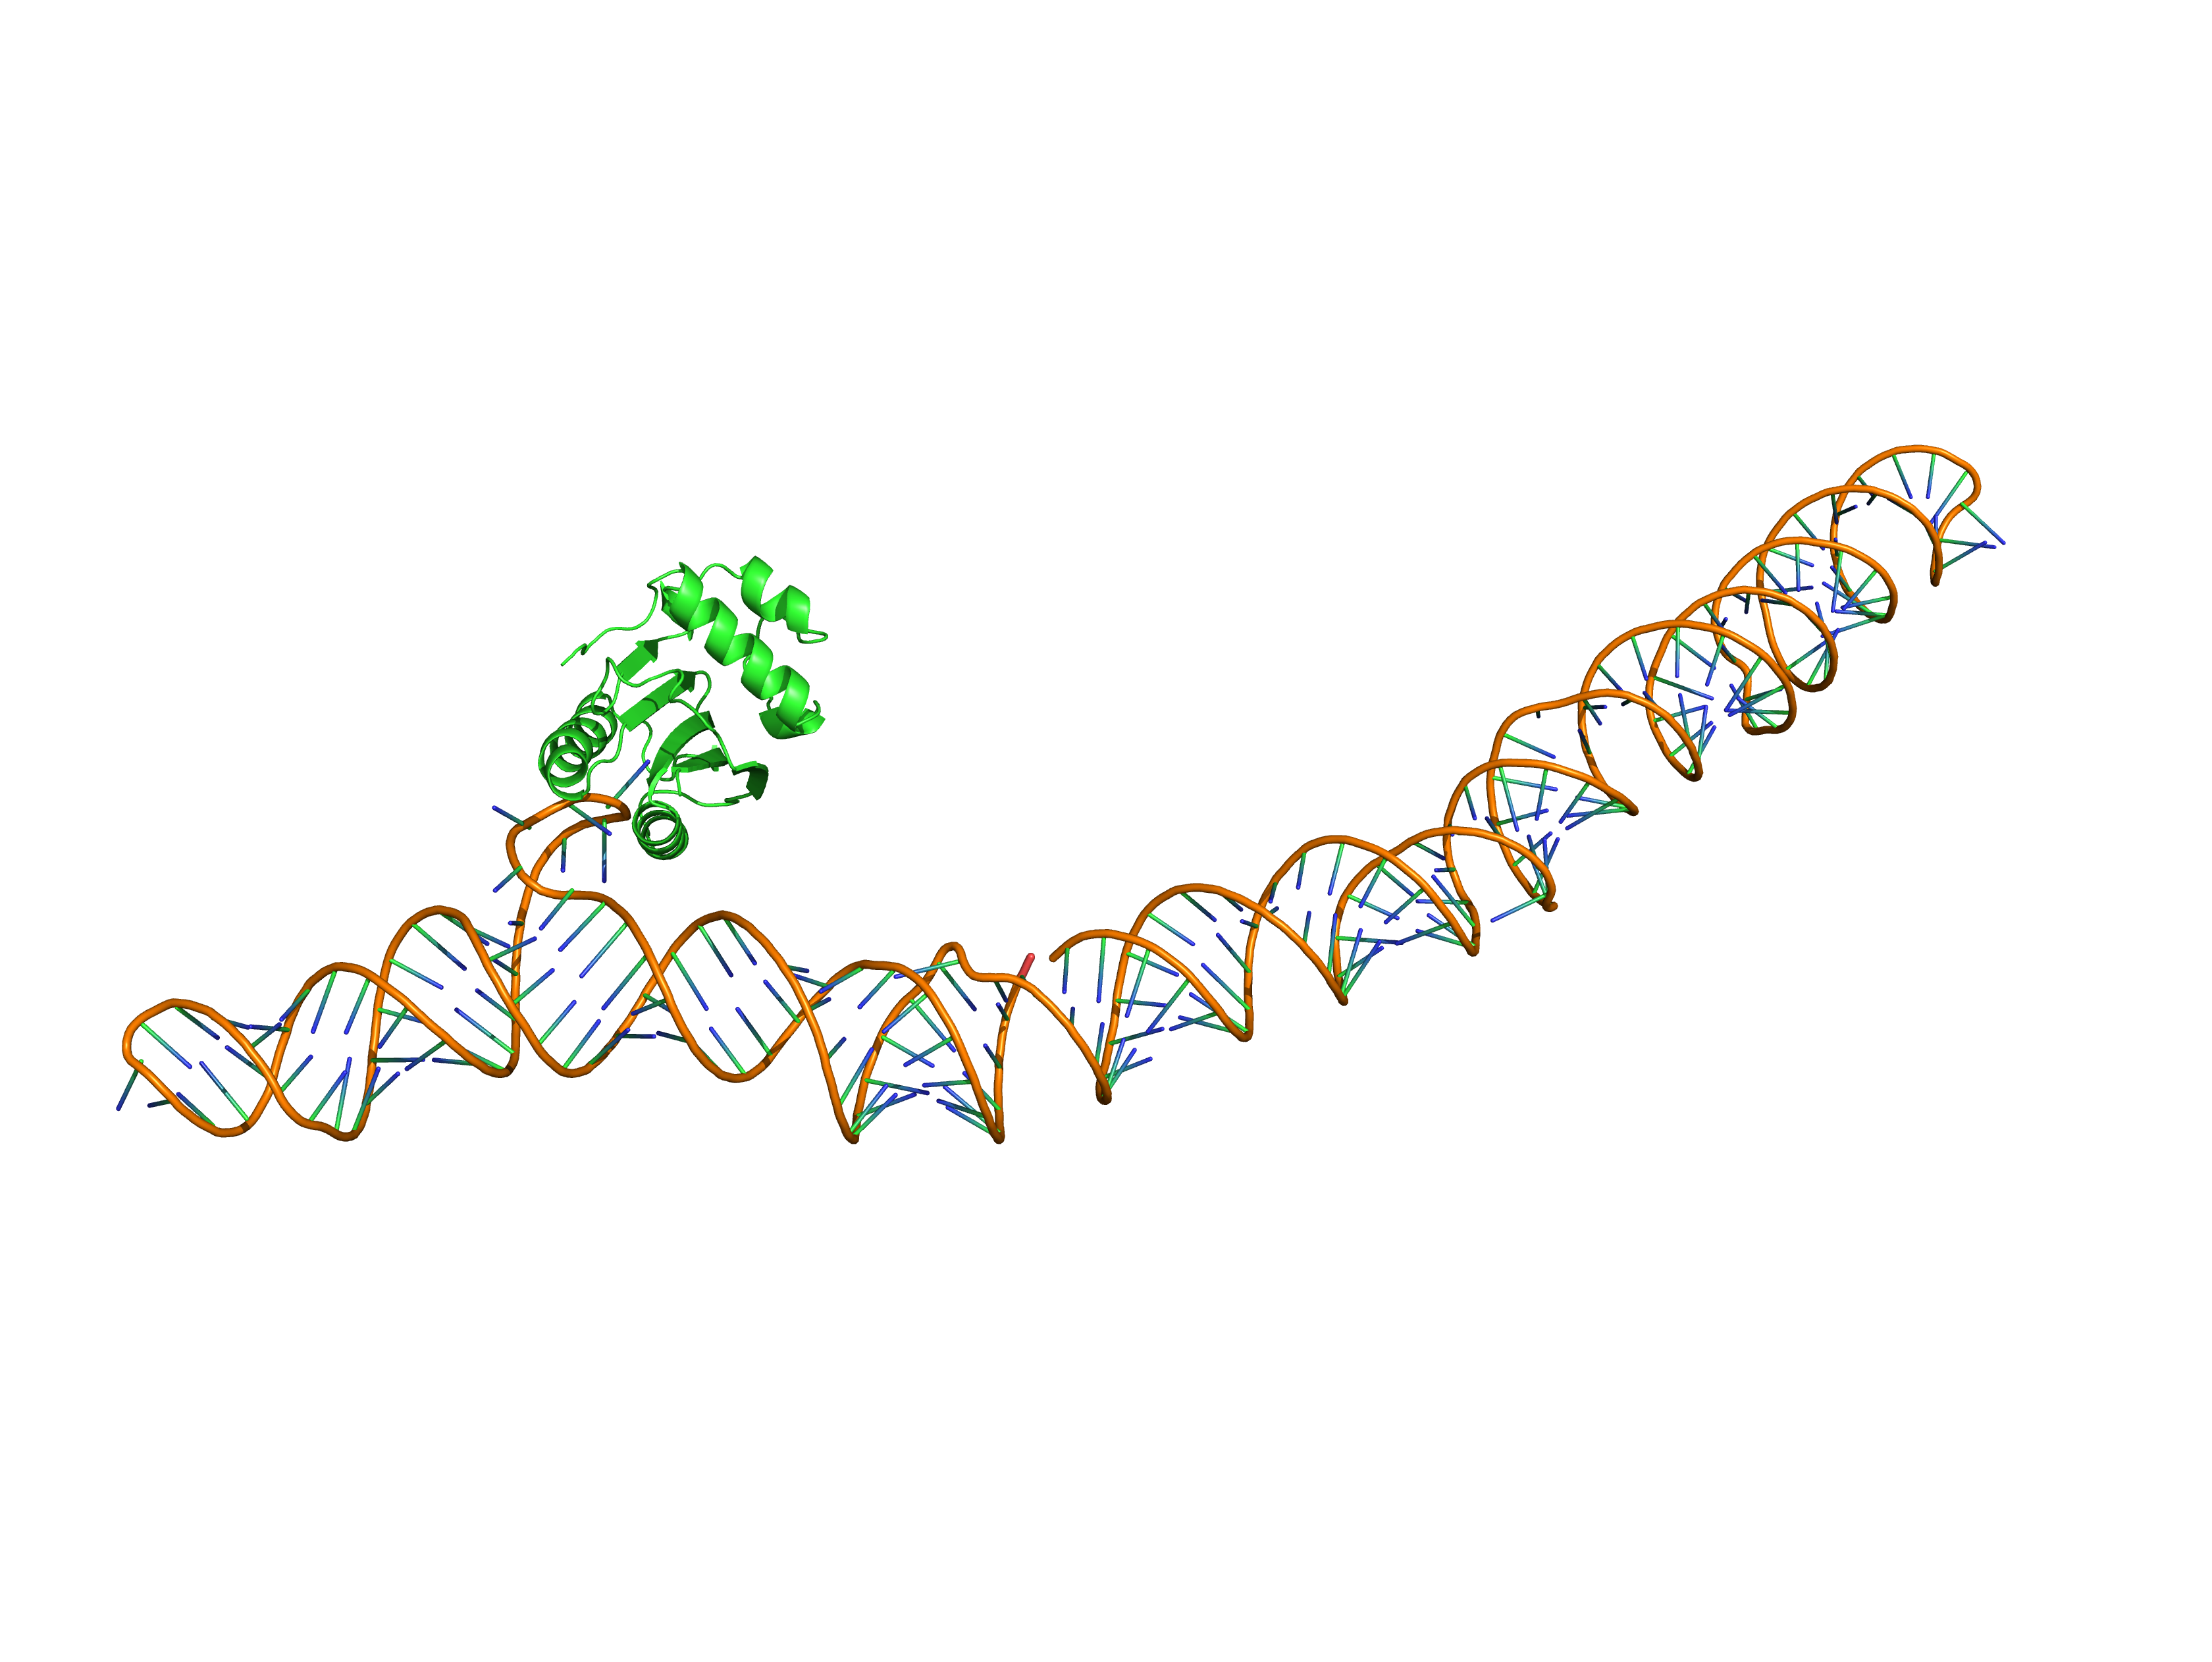
\includegraphics[width=\linewidth]{figures/results/cand332-BLUF-struct.png} 
    \end{subfigure}
    \caption[Predicted ribonucleoprotein complex structure]{\textbf{Predicted ribonucleoprotein complex structure of BLUF with identified RNA candidates.}
    Predicted structures of representative RNA and protein sequences from the two most promising structured RNA elements identified through the discovery pipeline.
    Predictions were made with AlphaFold 3 and the highest-confidence model is shown.
    \textbf{(a)} shows the predicted structure and interaction of candidate 130 with the \ac{BLUF} containing protein it was found near,
    \textbf{(b)} shows that for candidate 332.}
    \label{fig:bluf-rnp}
\end{figure}

RNA binding is predicted around the \ac{BLUF} \ac{FAD} binding site identified by \citet{Kita2005}, although these predictions are low confidence (see below).
Appendix Figure~\ref{fig:bluf-rnp-negative-control} shows the predicted structure of the \ac{BLUF} domain with a negative control RNA, which has no documented relationship to the \ac{BLUF} domain.
It predicted an interaction with the protein domain, albeit at a different site to the candidates identified by the discovery pipeline.
A positive control was also run with the Bridge RNA and Chain C, IS621 transposase, found by \citet{Durrant2024} to interact with the Bridge RNA.
The predicted structure is shown in Appendix Figure~\ref{fig:bridge-rna-rnp-positive-control}.
This shows a clearer interaction with multiple predicted binding sites.

\ac{ipTM} scores are an output measure of confidence from the prediction algorithm quantifying the interaction prediction confidence between the two molecules, with a score of 1 indicating high confidence and a score of 0 indicating low confidence.
The \ac{ipTM} scores for the two candidates 130 and 332 are 0.22 and 0.08, respectively.
Comparatively, the score for the positive control is 0.26 and that of the negative control is 0.1.
These scores are all low: candidate 130 (0.22) is only slightly above the negative control (0.1) and below even the Bridge RNA positive control (0.26), and candidate 332 (0.08) is below the negative control.
Neither prediction therefore provides evidence of a specific interaction between the candidates and the \ac{BLUF} domain.
[NOTE: consider adding, with a citation, that ipTM values below about 0.6 are generally regarded as low confidence.]

\section{Covariance model clustering}

Clustering covariance models (CMs) requires a pairwise score that is both reliable and statistically robust, so that a distance between two models can be interpreted rather than just ranked. 
This section describes how candidate scoring approaches were benchmarked against Rfam clans, and how the chosen approach was then applied to cluster the positive control candidates.

Rfam groups families into clans on the basis of shared evolutionary origin, which makes clan membership a useful, if imperfect, ground truth for benchmarking: models in the same clan should recognise each other's sequences, whereas models from different clans should not. 
Rfam clan membership was therefore used to benchmark the pairwise scoring methods.

\subsection{Clustering approaches}

Three approaches were tested: one which searched for a common ancestor with a genetic algorithm, one which used the median bit scores of sequence populations between the models, and one which looked for distributional differences between the models' sequence population bit score distributions. 
The clan benchmark test took roughly 11 hours over 64 \ac{CPU} cores, while the median bit score and distributional difference approaches took roughly 7 hours over 64 \ac{CPU} cores. [NOTE: clarify which approach took about 11 hours. Presumably the optimal sequence approach, versus about 7 hours for the other two.]
Each was evaluated on its ability to distinguish within-clan pairs from all other pairs (Table~\ref{tab:classifier_comparison}).

\begin{table}[htbp]
\centering
\footnotesize
\caption[Comparison of pairwise scoring approaches on Rfam clans]{\textbf{Separation of within-clan from other pairs by each scoring approach.} 
Within-clan ($n = 27$) and other ($n = 919$) pairs from annotated Rfam entries. 
AUC is the probability that a randomly chosen within-clan pair scores higher than a randomly chosen other pair.
Confidence intervals were obtained by bootstrapping over families, to account for each family appearing in many pairs.}
\label{tab:classifier_comparison}
\begin{tabular}{lccc}
\hline
\textbf{Approach} & \textbf{Statistic} & \textbf{AUC} & \textbf{95 \% CI} \\
\hline
Common ancestor (similarity ratio) & similarity ratio & 0.832 & [0.716 -- 0.934] \\
Median bit score vs.\ null & summed medians & 0.767 & [0.560 -- 0.944] \\
KS distribution vs.\ null & $D_{A\rightarrow B} + D_{B\rightarrow A}$ & 0.835 & [0.653 -- 0.957] \\
\hline
\end{tabular}
\end{table}

All three approaches gave moderate separation of within-clan pairs from other pairs. 
The similarity ratio and the summed \ac{KS} statistic performed almost identically (AUC = 0.832 and 0.835), while the summed median bit score against the null performed less well (AUC = 0.767). [NOTE: report the 95 percent bootstrap confidence intervals described in Methods.] 
Because the \ac{KS} approach provides a per-pair test against a null distribution, which the similarity ratio does not, it was used for all remaining analyses.

\subsection{Distributional differences to the null}

The \ac{KS} approach compares the bit scores obtained when one model scores the sequences of another against a null distribution of shuffled sequences, in each direction. 
Figure~\ref{fig:ks-worked-example} shows this for two pairs. 

\begin{figure}[H]
    \centering
    \begin{subfigure}[t]{0.45\textwidth}
        \centering
        \caption{}
        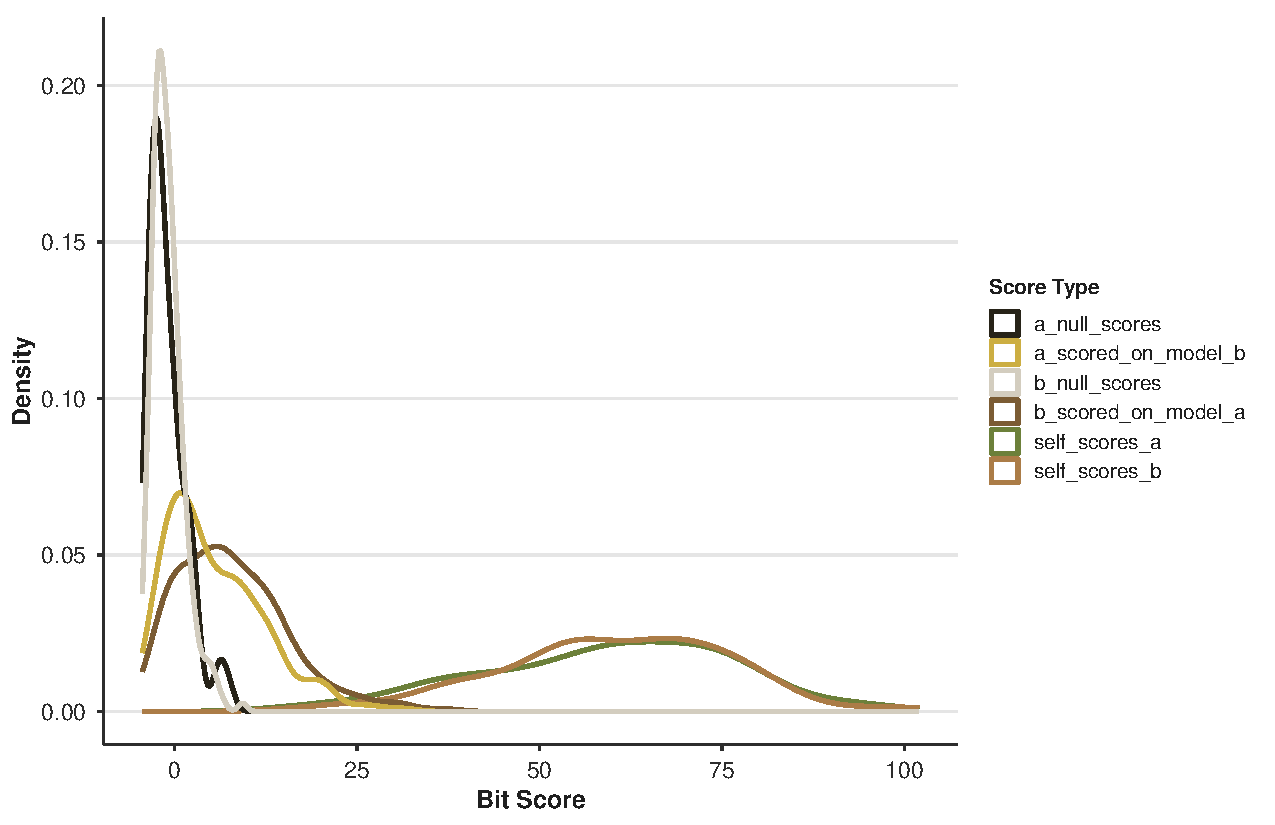
\includegraphics[width=\linewidth]{figures/results/cm-simile/SNORA17_SNORA43_distribution.pdf}
        \label{fig:snora17-snora43-dist}
    \end{subfigure}
    \hfill
    \begin{subfigure}[t]{0.45\textwidth}
        \centering
        \caption{}
        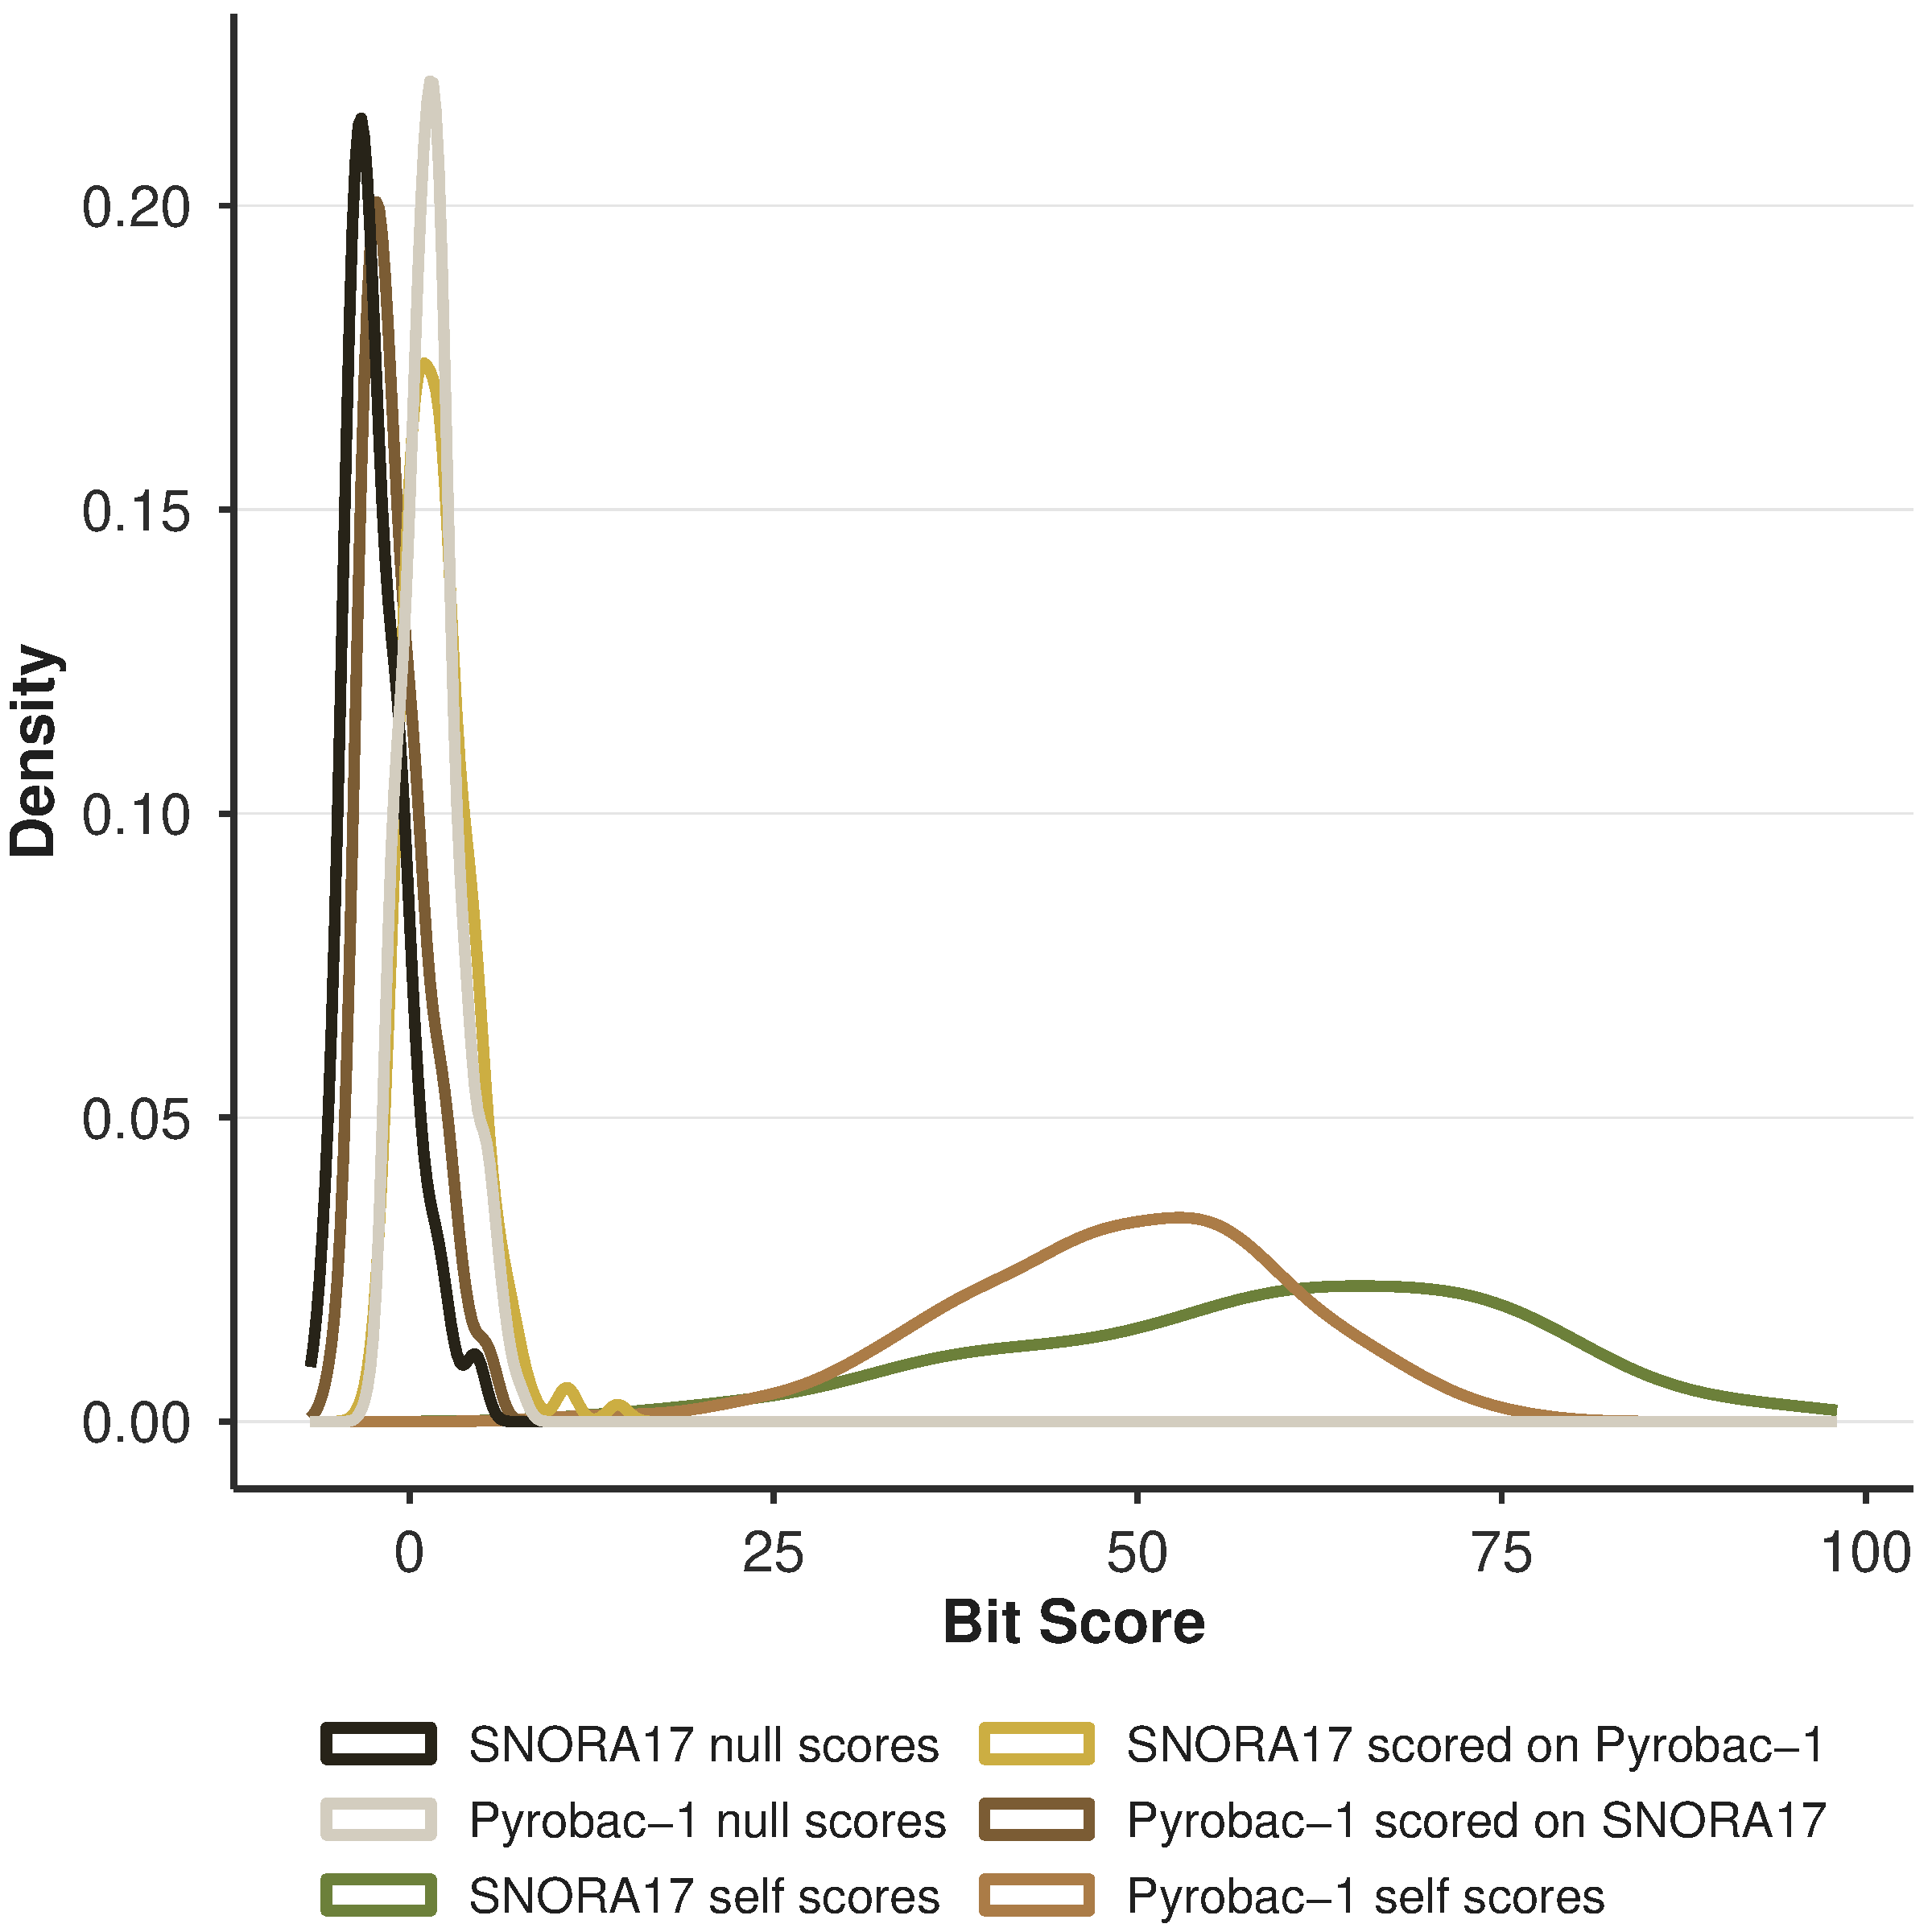
\includegraphics[width=\linewidth]{figures/results/cm-simile/SNORA17_Pyrobac-1_distribution.pdf}
        \label{fig:snora17-pyrobac-dist}
    \end{subfigure}

    \caption[Distributional comparison for a within-clan and a between-clan model pair]{\textbf{Distributional comparison of bitscores for a within-clan and a between-clan model pair.} 
    Cross comparison bit score distributions are compared to null sequence distributions.
    Self bit scores (sequences scored against their model of origin) are shown for comparison.
    \textbf{(a)}: SNORA17 vs.\ SNORA43, both members of the same clan; the cross-comparison distribution (SNORA43 sequences scored against the SNORA17 model) is compared to null sequences (KS $D=0.673$, $p=1.66\times10^{-19}$ scored against SNORA43; $D=0.557$, $p=3.22\times10^{-30}$ scored against SNORA17). 
    \textbf{(b)}: SNORA17 vs.\ Pyrobac-1, from different clans;  (KS $D=0.263$, $p=5.26\times10^{-7}$; $D=0.112$, $p=0.112$). 
    ($N = 300$ emitted sequences per model)}
    \label{fig:ks-worked-example}
\end{figure}

The distributions for the within-clan pair (SNORA17 and SNORA43) are wider and shifted to higher bit scores than the null distribution of dinucleotide-shuffled sequences.
\ac{KS} tests are a measure of distributional difference, and make no assumptions about the shape of the distributions \citep{Smirnov1939}.
For SNORA17 and SNORA43, which belong to the same clan, the cross-comparison scores were strongly shifted from the null in both directions ($D = 0.673$ and $D = 0.557$; $p = 1.66 \times 10^{-19}$ and $3.22 \times 10^{-30}$). 
For SNORA17 and Pyrobac-1, which belong to different clans, the shift was much weaker in one direction ($D = 0.263$, $p = 5.26 \times 10^{-7}$) and not significant in the other ($D = 0.112$, $p = 0.112$).
Summing the two directional statistics therefore gives a single, symmetric measure of mutual recognition.

Across all pairs tested, the summed \ac{KS} statistic was significantly higher for within-clan pairs ($n = 27$) than for other pairs ($n = 919$; Wilcoxon $p = 2.76 \times 10^{-9}$; Figure~\ref{fig:ks-boxplot}). 
Because every model is compared against a single null population it is also considerably cheaper to compute than the bootstrap empirical-p value approach.

\begin{figure}[H]
    \centering
    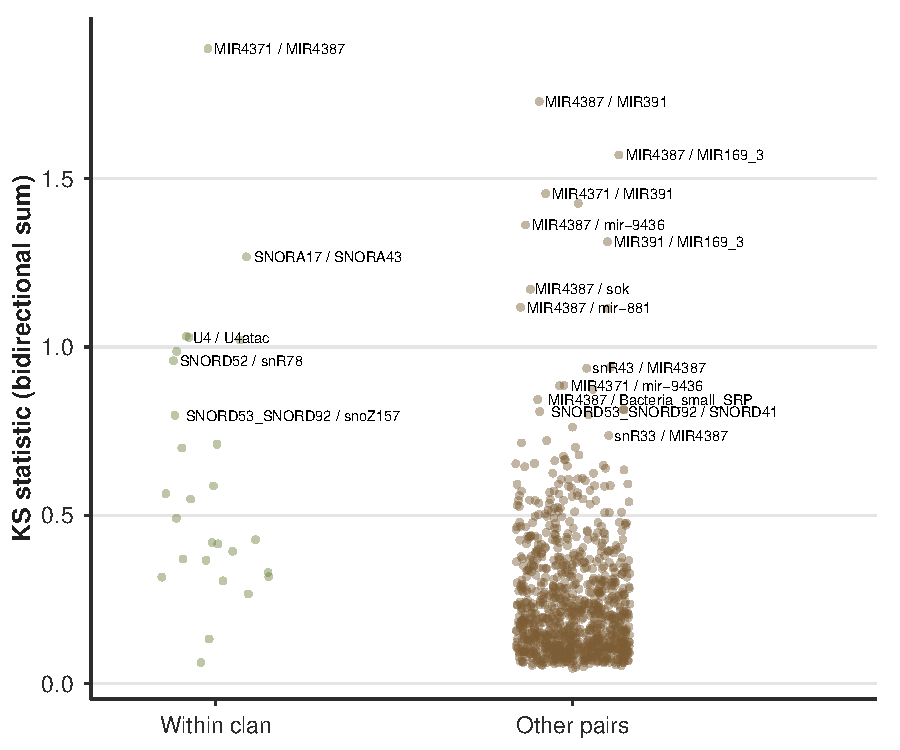
\includegraphics[width=0.9\textwidth]{figures/results/ks_ratio_jitterplot.pdf}
    \caption[Within- vs.\ between-clan separation using the KS statistic against a single null population]
    {\textbf{Within- vs.\ between-clan separation using the KS statistic compared against a single null population.} 
    The $y$-axis is the sum of the two two-sample KS statistics, $D$, of the bit score distribution against the null (both $D_{A \rightarrow B}$ and $D_{B \rightarrow A}$).
    A pair is labelled within-clan ($n = 27$) if both families belong to the same Rfam clan, and other ($n = 919$) otherwise, including pairs involving a family with no clan assignment.
    Top 3\% of pairs are labelled with the family names.
    ($N = 300$ emitted sequences per model)}
    \label{fig:ks-boxplot}
\end{figure}

\subsection{Clustering positive control candidates}

The summed \ac{KS} statistic was used to cluster the candidate models together with the FMN riboswitch model (\texttt{RF00050}) and a model built from the consensus model and the same flanking sequences as the candidates (\texttt{FMN\_on\_micro}), using the distance $2 - (D_{A \rightarrow B} + D_{B \rightarrow A})$ and average-linkage hierarchical clustering (Figure~\ref{fig:candidate-clustering}). 
The resulting tree shows candidates clustering into three main groups, one with the consensus FMN riboswitch model clustering with the (\texttt{FMN\_on\_micro}) model and candidates 539, 384, 491, 416, 40, 531, 379, 35 and 647.
These close candidates are also the candidates with the highest coordinate overlap identity to the true-positive alignment (Table~\ref{tab:rscape_summary}).
Candidates 442, 109 and 396 do not cluster with the FMN riboswitch model, and are therefore likely to be distinct from the true-positive alignment.
109 and 396 cluster together, which can also be observed from their predicted secondary structures (Appendix Figure~\ref{fig:drh-appendix-structures-2}).
In downstream analysis these candidates could be combined into a single model, potentially improving the alignment and covariation signal. [NOTE: the Discussion says attempts to combine covariance models were unsuccessful. Link to that here or reword.]

The (\texttt{FMN\_on\_micro}) model was constructed with the same iterative expansion approach as the candidates, but using the Rfam \ac{FMN} riboswitch model to identify sequences in the same flanking regions as the candidates.
Through this iterative expansion approach the structure of the input model is preserved.
The resulting model is measured to be more similar to the Rfam model than the candidates (Figure~\ref{fig:cluster-dendrogram}), although it was built from a wider range of sequences.
Seed alignment analysis revealed that similar seed alignments were used to build the candidates and the (\texttt{FMN\_on\_micro}) model (Table~\ref{tab:rscape_summary}).
The closer clustering of the (\texttt{FMN\_on\_micro}) model with the Rfam model than with the candidates may indicate sensitivity of the clustering approach to structural differences, but could also reflect shared construction, since structure is carried through from the Rfam model during iterative expansion.
A control, such as building an \ac{FMN} model de novo from the same sequences, would distinguish these possibilities.

\begin{figure}[H]
    \centering
    \begin{subfigure}[b]{0.6\textwidth}
        \centering
        \caption{}
        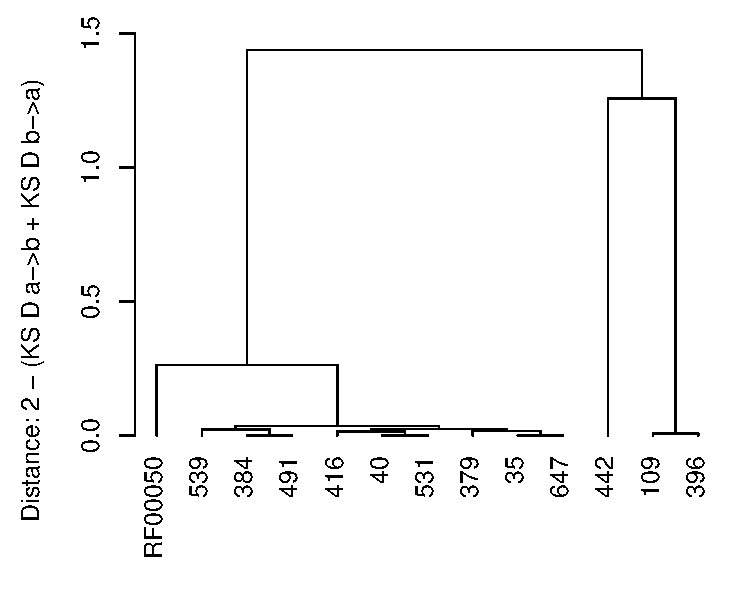
\includegraphics[width=\textwidth]{figures/results/candidate_clustering_dendrogram.pdf}
        \label{fig:cluster-dendrogram}
    \end{subfigure}
    \hfill
    \begin{subfigure}[b]{0.6\textwidth}
        \centering
        \caption{}
        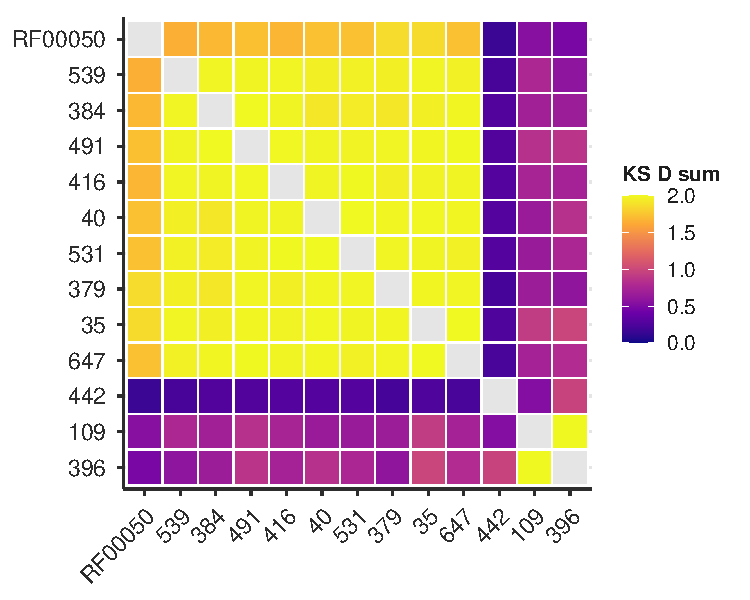
\includegraphics[width=\textwidth]{figures/results/candidate_clustering_heatmap.pdf}
        \label{fig:cluster-heatmap}
    \end{subfigure}
    \caption[Clustering of candidate covariance models by cross-recognition]{%
    \textbf{Clustering of candidate covariance models by cross-recognition.}
    \textbf{(a)} Hierarchical clustering (average linkage) of the candidate models, the Rfam consensus FMN riboswitch model (\texttt{RF00050}) and a model built from the consensus model and the same flanking sequences as the candidates (\texttt{FMN\_on\_micro}), 
    using the distance $2 - (D_{A \rightarrow B} + D_{B \rightarrow A})$, where $D$ is the two-sample Kolmogorov--Smirnov statistic against the shuffled null in each direction. 
    \textbf{(b)} Pairwise summed KS statistic, with models ordered as in (a); higher values indicate that the two models recognise each other's sequences more strongly.
    Candidates are labelled by cluster number.
    ($N = 300$ emitted sequences per model)
    }
    \label{fig:candidate-clustering}
\end{figure}
